\newcommand{\anhangText}{
	% Gibt es nicht
}

\newcommand{\anhangEins}{
	\paragraph{Detaillierte Zeitplanung}
	Hier könnte ihre Tabelle abgebildet sein
}

\newcommand{\anhangZwei}{
	\paragraph{Wasserfall-Modell}
	\begin{figure}[ht]
		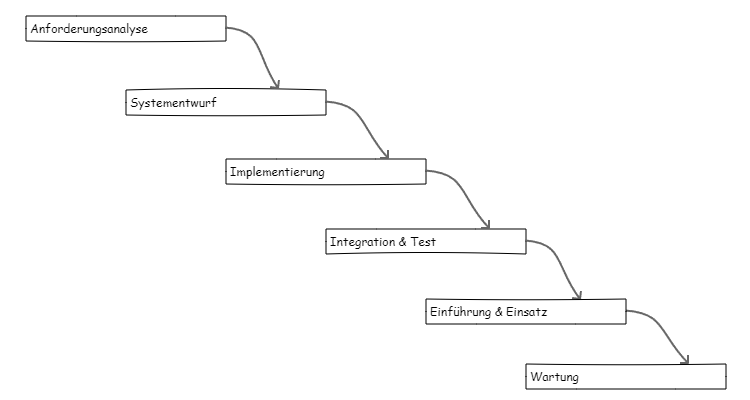
\includegraphics[width=13cm]{img/Wasserfallmodell.png}
		\caption{Darstellung des geplanten Wasserfall-Modells}
	\end{figure}
	\label{fig:wasserfallmodell}
}

\newcommand{\anhangDrei}{
	\paragraph{Programmstruktur}
	\begin{figure}[ht]
		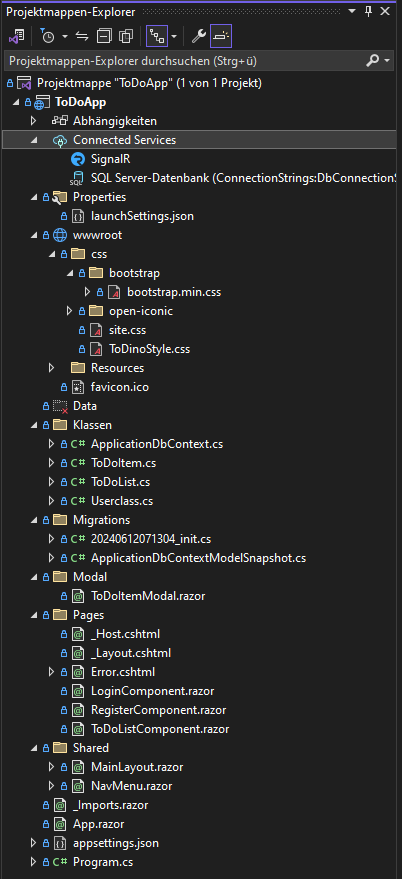
\includegraphics[width=13cm]{img/A3Abb2.png}
		\caption{Visual Studio Programmstruktur}
	\end{figure}
	\label{fig:programmstruktur}
}

\newcommand{\anhangVier}{
	\paragraph{To-Dino Seite}
	\begin{figure}[ht]
		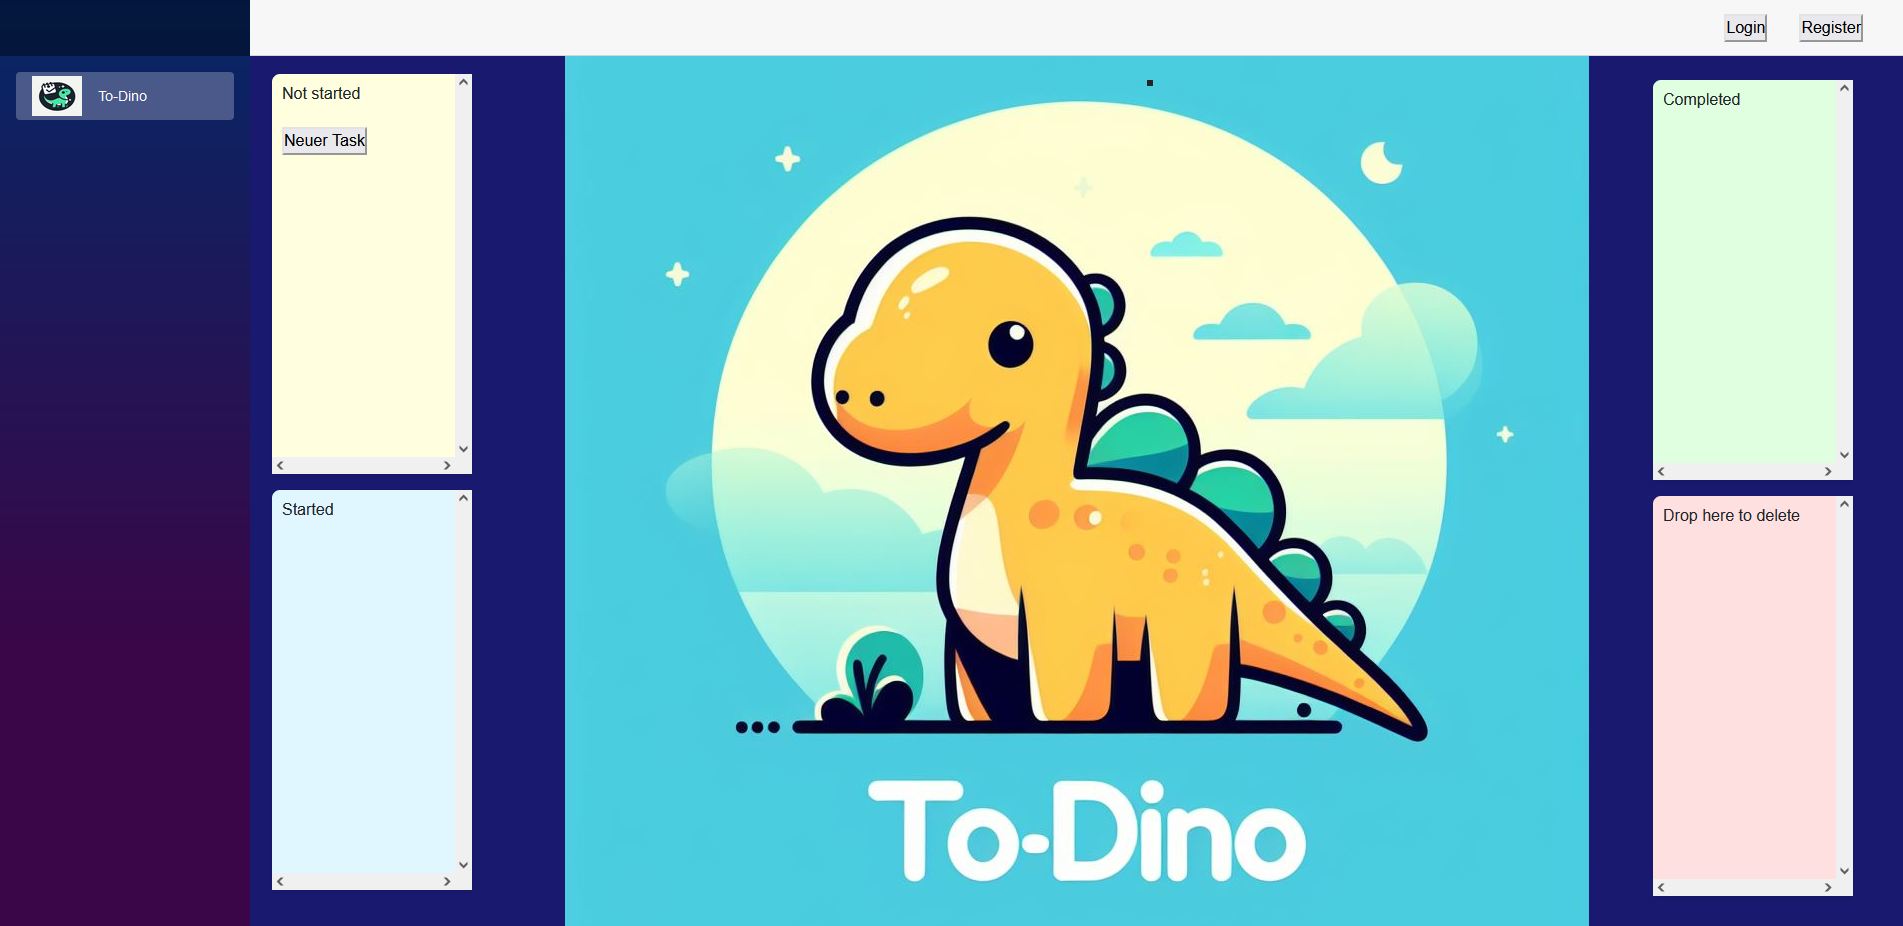
\includegraphics[width=13cm]{img/A4Abb3.png}
		\caption{Darstellung der implementierten To-Dino Seite}
	\end{figure}
	\label{fig:todinoseite}
}

\newcommand{\anhangFuenf}{
	\paragraph{Komponenten der Hauptseite}
	\begin{figure}[ht]
		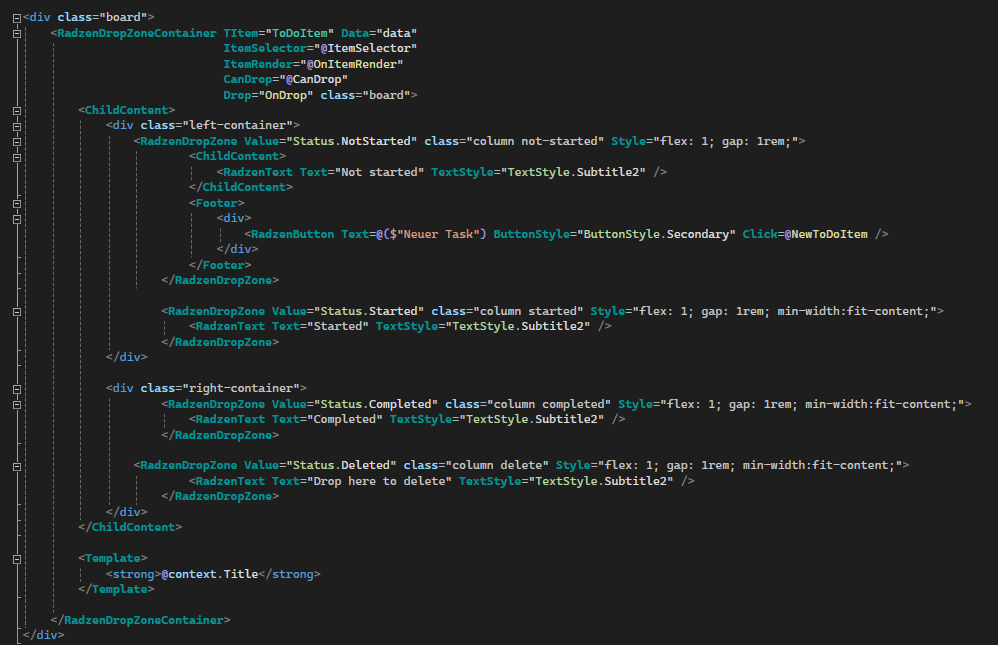
\includegraphics[width=13cm]{img/A5Abb4.png}
		\caption{Die integrierten Blazor.Radzen Komponenten}
	\end{figure}
	\label{fig:hauptseitekomponenten}
}

\newcommand{\anhangSechs}{
	\paragraph{Hauptseiten Code-Block}
	\begin{figure}[ht]
		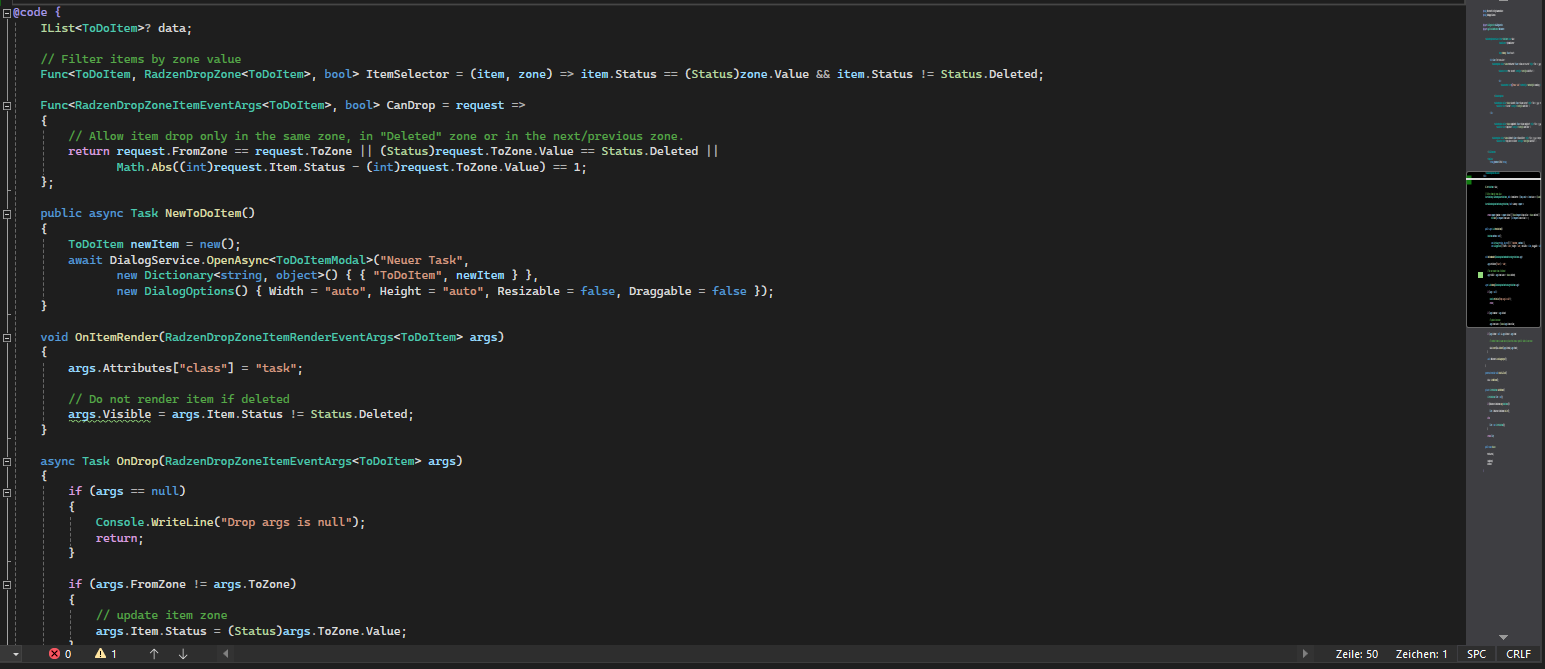
\includegraphics[width=13cm]{img/A6Abb5.png}
		\caption{Darstellung des geplanten Wasserfall-Modells}
	\end{figure}
	\label{fig:hauptseitecodeblock}
}

\newcommand{\anhangSieben}{
	\paragraph{ToDoItem-Klasse}
	\begin{figure}[ht]
		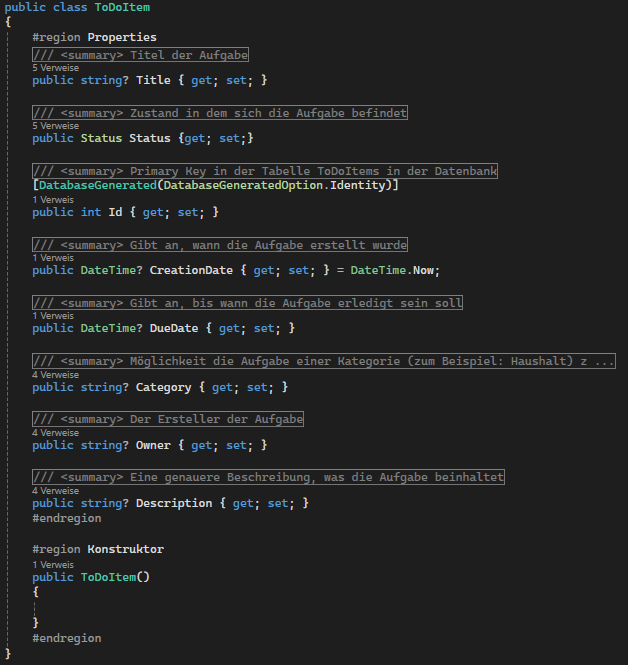
\includegraphics[width=13cm]{img/A7Abb6.png}
		\caption{Implementierung der Klasse 'ToDoItem'}
	\end{figure}
	\label{fig:todoitemklasse}
}

\newcommand{\anhangZehn}{
	\paragraph{ApplicationDbContext-Klasse}
	\begin{figure}[ht]
		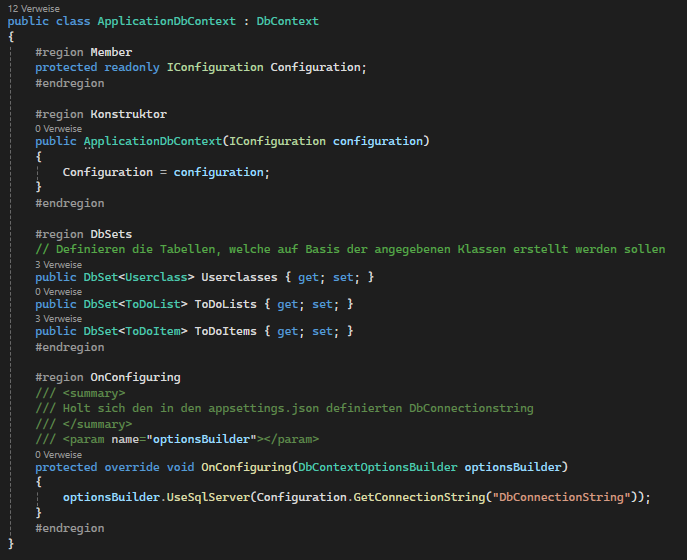
\includegraphics[width=13cm]{img/A10Abb9.png}
		\caption{Implementierung der Klasse 'ApplicationDbContext'}
	\end{figure}
	\label{fig:applicationdbcontext}
}